\section{Specifications}
\label{sec:specs}
\newcounter{SpecID}

\subsection{Markers}
\refstepcounter{SpecID}
\label{spec:markers}

The arena is labelled with fiducial markers. Each marker number is associated
with a particular feature in the arena, and also has an associated size.
The marker numbers and sizes are as follows:

\begin{center}
\begin{tabular}{lcc}
  \toprule
  \textbf{Item} & \textbf{Marker Number} & \textbf{Marker Size (\si{mm})} \\
  \midrule
  Arena boundary & 0 -- 27 & 250 \\
  Central reservation & 28 -- 39 & 250  \\
  % 28 to 31 reserved for robot badges
  \bottomrule
\end{tabular}
\end{center}

All markers are oriented vertically such that the principal corner of the marker
(which is indicated by a dark grey dot in the black marker border) is on the
higher edge.

\subsection{Arena}
\refstepcounter{SpecID}
\label{spec:arena}

\begin{enumerate}
  \item The arena floor is an \SI{8}{m} $\times$ \SI{8}{m} square. The tolerance
        of these two dimensions is $\pm$ \SI{250}{mm}.
  \item The floor of the arena is carpeted.
  \item The layout of the arena is given in Figure~\ref{fig:arena}.
  \item The outer walls of the arena are at least \SI{600}{mm} high, and the
        interior surface is white plastic-coated hardboard.
  \item Each wall of the arena features seven \SI{250}{mm} fiducial markers.
        The positions of these markers is given in Figure~\ref{fig:sidewall}.
        The marker numbering is given in Figure~\ref{fig:arena}.
  \item The robot starting zones are squares which share corners with the arena
        itself. Their sides are of length \si{1}{m}.
  \item In the centre of the arena is a central reservation raised by
        at least \SI{250}{mm} above the arena floor. It is square, and
        sized such that the width of the track is \SI{2}{m}.
  \item The track boundaries are visually delineated on the floor of the arena
        by tape. The actual boundary is on the trailing edge of the tape --
        that is, a robot has passed the boundary when the back of the robot
        is past the tape.
\end{enumerate}

\begin{sidewaysfigure}
  \includegraphics[scale=0.58]{fig-sidewall.pdf}
  \caption{Layout of markers along each arena wall.}
  \label{fig:sidewall}
\end{sidewaysfigure}

\begin{figure}
  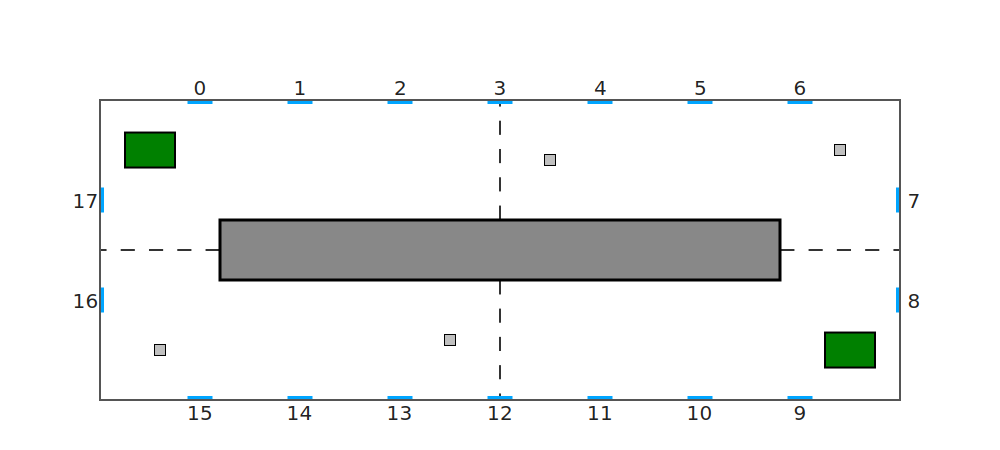
\includegraphics[scale=0.58]{fig-arena.pdf}
  \caption{Layout zones and cans in the arena.}
  \label{fig:arena}
\end{figure}

\subsection{Tin Cans}
\refstepcounter{SpecID}
\label{spec:cans}

\begin{enumerate}
  \item The tin cans are standard steel cans. Size and weight TBD.
  \item The initial layout of tin cans in the arena is given in
        Figure~\ref{fig:arena}.
\end{enumerate}

